\documentclass{standalone}
\usepackage{tikz}
\usetikzlibrary{patterns, positioning}
\usepackage[sfdefault]{ClearSans} %% option 'sfdefault' activates Clear Sans as the default text font
\usepackage[T1]{fontenc}

\begin{document}
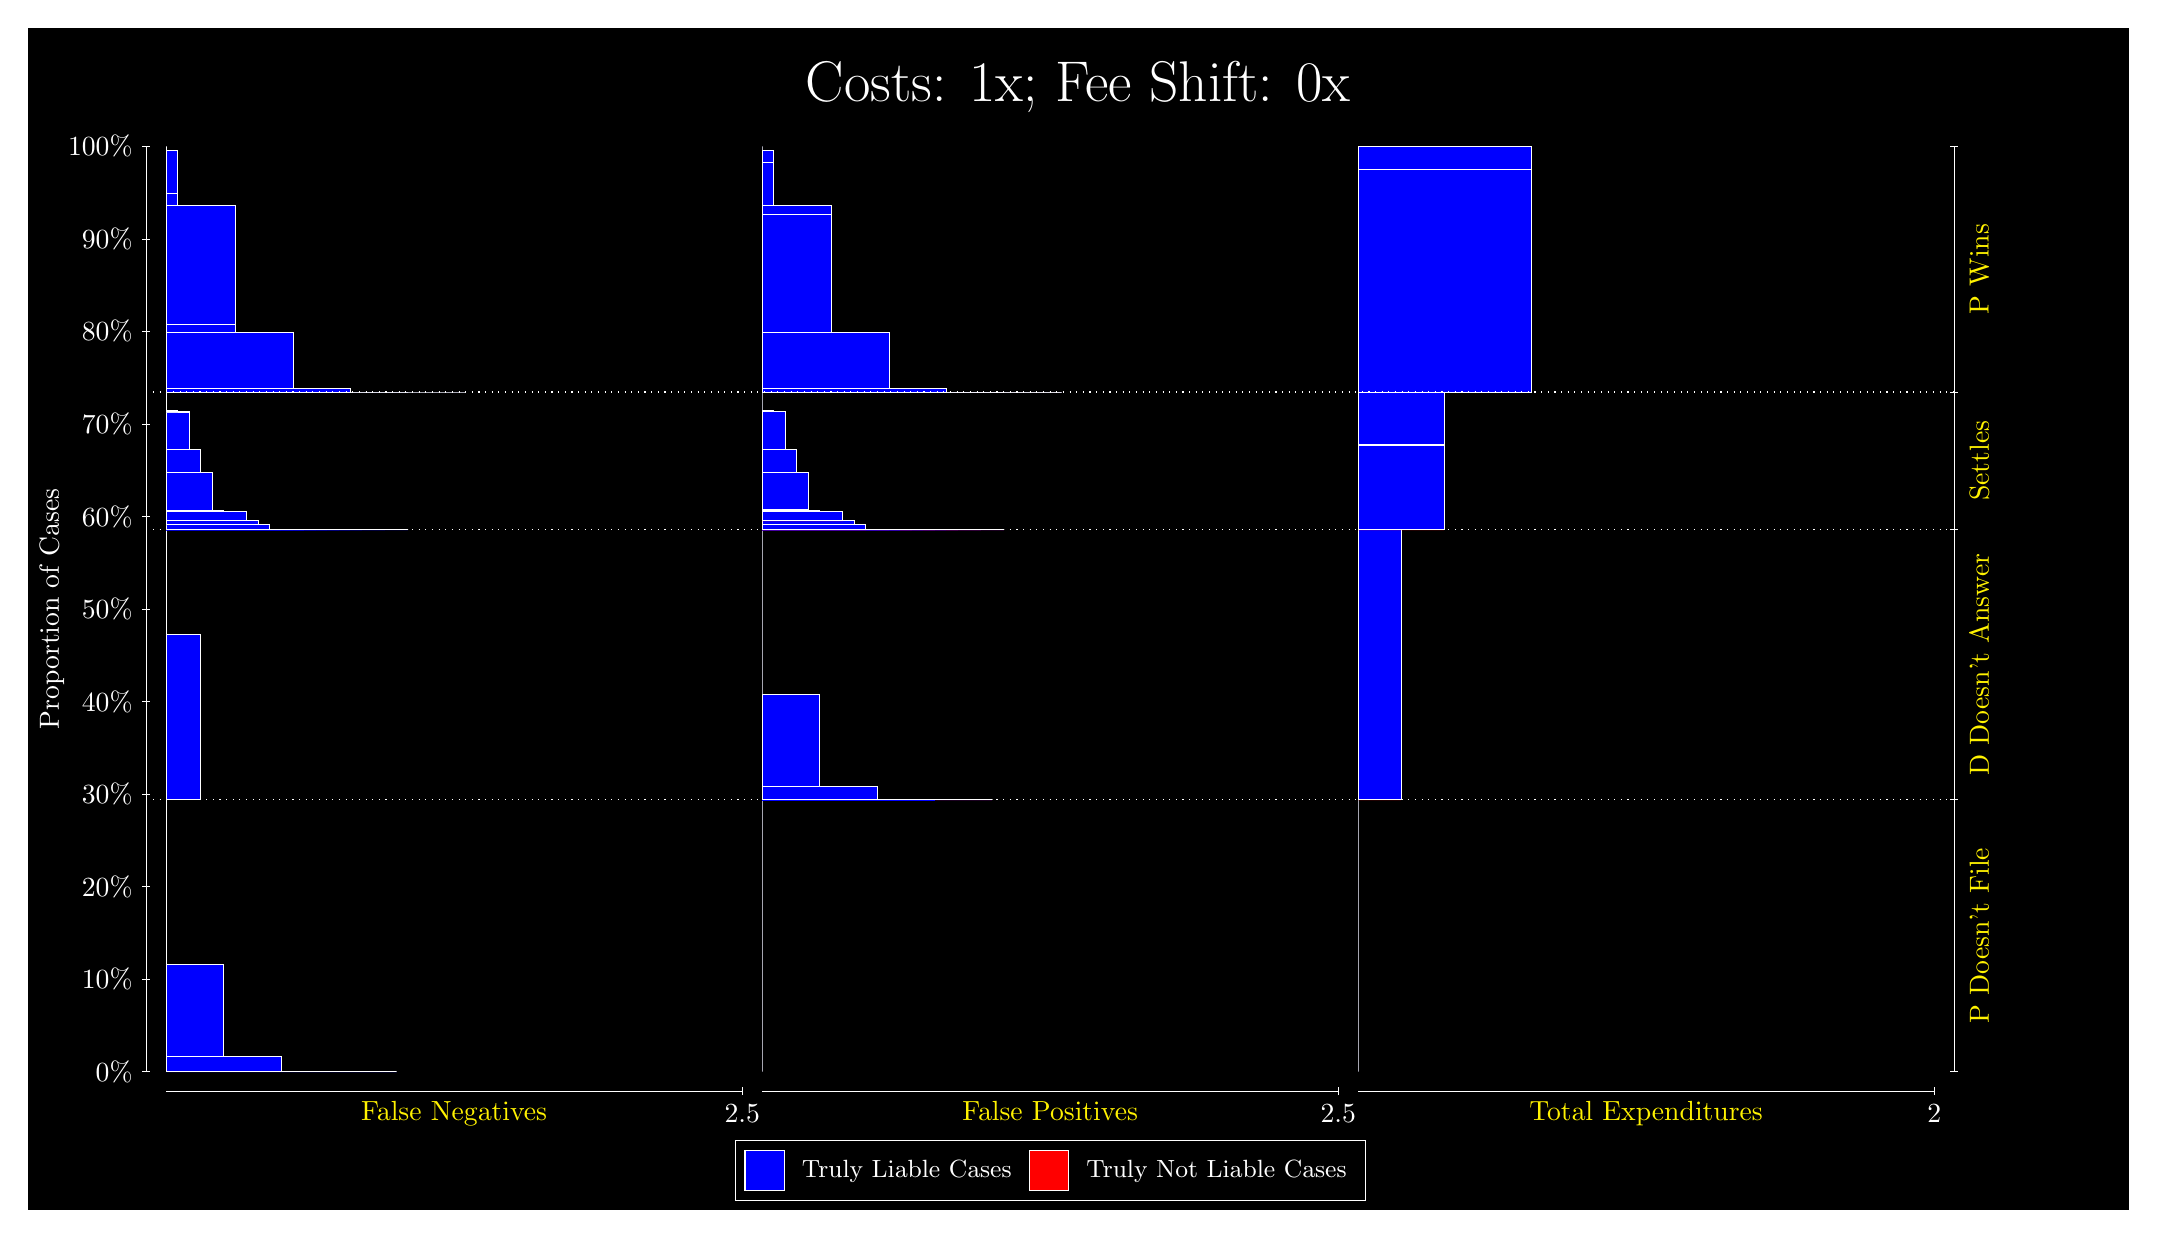
\begin{tikzpicture}
\draw[fill=black] (0,0) rectangle (26.667,15);
\draw[text=white] (0,13.5) rectangle (26.667,15) node[midway] {\huge Costs: 1x; Fee Shift: 0x};
\draw[white, very thin] (1.5,1.75) -- (1.5,13.5);
\node[rotate=90, text=white, anchor=center] at (0.3, 7.625) {Proportion of Cases};
\draw[white, very thin] (1.45,1.75) -- (1.55,1.75);
\node[text=white, anchor=east] at (1.45, 1.75) {0\%};
\draw[white, very thin] (1.45,2.925) -- (1.55,2.925);
\node[text=white, anchor=east] at (1.45, 2.925) {10\%};
\draw[white, very thin] (1.45,4.1) -- (1.55,4.1);
\node[text=white, anchor=east] at (1.45, 4.1) {20\%};
\draw[white, very thin] (1.45,5.275) -- (1.55,5.275);
\node[text=white, anchor=east] at (1.45, 5.275) {30\%};
\draw[white, very thin] (1.45,6.45) -- (1.55,6.45);
\node[text=white, anchor=east] at (1.45, 6.45) {40\%};
\draw[white, very thin] (1.45,7.625) -- (1.55,7.625);
\node[text=white, anchor=east] at (1.45, 7.625) {50\%};
\draw[white, very thin] (1.45,8.8) -- (1.55,8.8);
\node[text=white, anchor=east] at (1.45, 8.8) {60\%};
\draw[white, very thin] (1.45,9.975) -- (1.55,9.975);
\node[text=white, anchor=east] at (1.45, 9.975) {70\%};
\draw[white, very thin] (1.45,11.15) -- (1.55,11.15);
\node[text=white, anchor=east] at (1.45, 11.15) {80\%};
\draw[white, very thin] (1.45,12.325) -- (1.55,12.325);
\node[text=white, anchor=east] at (1.45, 12.325) {90\%};
\draw[white, very thin] (1.45,13.5) -- (1.55,13.5);
\node[text=white, anchor=east] at (1.45, 13.5) {100\%};

\draw[white, very thin] (24.457,1.75) -- (24.457,13.5);
\draw[white, very thin] (24.407,1.75) -- (24.507,1.75);
\node[anchor=west] at (24.407, 1.75) {};
\draw[white, very thin] (24.407,5.2024) -- (24.507,5.2024);
\node[anchor=west] at (24.407, 5.2024) {};
\draw[white, very thin] (24.407,8.633) -- (24.507,8.633);
\node[anchor=west] at (24.407, 8.633) {};
\draw[white, very thin] (24.407,10.38) -- (24.507,10.38);
\node[anchor=west] at (24.407, 10.38) {};
\draw[white, very thin] (24.407,13.5) -- (24.507,13.5);
\node[anchor=west] at (24.407, 13.5) {};

\draw[white, very thin, fill=blue] (1.75,1.75) rectangle (4.6775,1.75);
\draw[white, very thin, fill=blue] (1.75,1.75) rectangle (3.9457,1.7516);
\draw[white, very thin, fill=blue] (1.75,1.7516) rectangle (3.2138,1.9396);
\draw[white, very thin, fill=blue] (1.75,1.9396) rectangle (2.4819,3.107);
\draw[white, very thin, fill=red] (1.75,3.107) rectangle (1.75,3.107);
\draw[white, very thin, fill=blue] (1.75,3.107) rectangle (1.75,5.2024);
\draw[white, very thin, fill=blue] (1.75,5.2024) rectangle (2.1891,7.2979);
\draw[white, very thin, fill=red] (1.75,7.2979) rectangle (1.75,7.2979);
\draw[white, very thin, fill=blue] (1.75,7.2979) rectangle (1.75,8.633);
\draw[white, very thin, fill=blue] (1.75,8.633) rectangle (4.8239,8.633);
\draw[white, very thin, fill=blue] (1.75,8.633) rectangle (4.5312,8.633);
\draw[white, very thin, fill=blue] (1.75,8.633) rectangle (4.2384,8.633);
\draw[white, very thin, fill=blue] (1.75,8.633) rectangle (4.092,8.633);
\draw[white, very thin, fill=blue] (1.75,8.633) rectangle (3.9457,8.633);
\draw[white, very thin, fill=blue] (1.75,8.633) rectangle (3.7993,8.633);
\draw[white, very thin, fill=blue] (1.75,8.633) rectangle (3.6529,8.6331);
\draw[white, very thin, fill=blue] (1.75,8.6331) rectangle (3.5065,8.6333);
\draw[white, very thin, fill=blue] (1.75,8.6333) rectangle (3.3602,8.6333);
\draw[white, very thin, fill=blue] (1.75,8.6333) rectangle (3.2138,8.6333);
\draw[white, very thin, fill=blue] (1.75,8.6333) rectangle (3.0674,8.6953);
\draw[white, very thin, fill=blue] (1.75,8.6953) rectangle (3.0674,8.6954);
\draw[white, very thin, fill=blue] (1.75,8.6954) rectangle (2.921,8.7481);
\draw[white, very thin, fill=blue] (1.75,8.7481) rectangle (2.7746,8.8648);
\draw[white, very thin, fill=blue] (1.75,8.8648) rectangle (2.6283,8.8648);
\draw[white, very thin, fill=blue] (1.75,8.8648) rectangle (2.6283,8.8654);
\draw[white, very thin, fill=blue] (1.75,8.8654) rectangle (2.4819,8.8833);
\draw[white, very thin, fill=blue] (1.75,8.8833) rectangle (2.3355,9.3582);
\draw[white, very thin, fill=blue] (1.75,9.3582) rectangle (2.3355,9.3635);
\draw[white, very thin, fill=blue] (1.75,9.3635) rectangle (2.1891,9.6496);
\draw[white, very thin, fill=blue] (1.75,9.6496) rectangle (2.0428,10.124);
\draw[white, very thin, fill=blue] (1.75,10.124) rectangle (2.0428,10.13);
\draw[white, very thin, fill=blue] (1.75,10.13) rectangle (1.8964,10.13);
\draw[white, very thin, fill=blue] (1.75,10.13) rectangle (1.8964,10.147);
\draw[white, very thin, fill=blue] (1.75,10.147) rectangle (1.75,10.148);
\draw[white, very thin, fill=red] (1.75,10.148) rectangle (1.75,10.148);
\draw[white, very thin, fill=blue] (1.75,10.148) rectangle (1.75,10.38);
\draw[white, very thin, fill=blue] (1.75,10.38) rectangle (5.5558,10.38);
\draw[white, very thin, fill=blue] (1.75,10.38) rectangle (4.8239,10.38);
\draw[white, very thin, fill=blue] (1.75,10.38) rectangle (4.092,10.433);
\draw[white, very thin, fill=blue] (1.75,10.433) rectangle (3.3602,11.133);
\draw[white, very thin, fill=blue] (1.75,11.133) rectangle (2.6283,11.239);
\draw[white, very thin, fill=blue] (1.75,11.239) rectangle (2.6283,12.747);
\draw[white, very thin, fill=blue] (1.75,12.747) rectangle (1.8964,12.899);
\draw[white, very thin, fill=blue] (1.75,12.899) rectangle (1.8964,13.446);
\draw[white, very thin, fill=red] (1.75,13.446) rectangle (1.75,13.446);
\draw[white, very thin, fill=blue] (1.75,13.446) rectangle (1.75,13.5);
\draw[white, very thin, fill=red] (9.3189,1.75) rectangle (9.3189,1.75);
\draw[white, very thin, fill=blue] (9.3189,1.75) rectangle (9.3189,5.2024);
\draw[white, very thin, fill=red] (9.3189,5.2024) rectangle (12.246,5.2024);
\draw[white, very thin, fill=blue] (9.3189,5.2024) rectangle (12.246,5.2024);
\draw[white, very thin, fill=blue] (9.3189,5.2024) rectangle (11.515,5.2031);
\draw[white, very thin, fill=blue] (9.3189,5.2031) rectangle (10.783,5.3711);
\draw[white, very thin, fill=blue] (9.3189,5.3711) rectangle (10.051,6.5376);
\draw[white, very thin, fill=blue] (9.3189,6.5376) rectangle (9.3189,8.633);
\draw[white, very thin, fill=red] (9.3189,8.633) rectangle (12.393,8.633);
\draw[white, very thin, fill=blue] (9.3189,8.633) rectangle (12.393,8.633);
\draw[white, very thin, fill=red] (9.3189,8.633) rectangle (12.1,8.633);
\draw[white, very thin, fill=blue] (9.3189,8.633) rectangle (12.1,8.633);
\draw[white, very thin, fill=red] (9.3189,8.633) rectangle (11.807,8.633);
\draw[white, very thin, fill=blue] (9.3189,8.633) rectangle (11.807,8.633);
\draw[white, very thin, fill=blue] (9.3189,8.633) rectangle (11.661,8.633);
\draw[white, very thin, fill=red] (9.3189,8.633) rectangle (11.515,8.633);
\draw[white, very thin, fill=blue] (9.3189,8.633) rectangle (11.515,8.633);
\draw[white, very thin, fill=blue] (9.3189,8.633) rectangle (11.368,8.633);
\draw[white, very thin, fill=red] (9.3189,8.633) rectangle (11.222,8.633);
\draw[white, very thin, fill=blue] (9.3189,8.633) rectangle (11.222,8.6331);
\draw[white, very thin, fill=blue] (9.3189,8.6331) rectangle (11.075,8.6333);
\draw[white, very thin, fill=blue] (9.3189,8.6333) rectangle (10.929,8.6333);
\draw[white, very thin, fill=red] (9.3189,8.6333) rectangle (10.929,8.6333);
\draw[white, very thin, fill=blue] (9.3189,8.6333) rectangle (10.929,8.6333);
\draw[white, very thin, fill=blue] (9.3189,8.6333) rectangle (10.783,8.6333);
\draw[white, very thin, fill=blue] (9.3189,8.6333) rectangle (10.636,8.6333);
\draw[white, very thin, fill=red] (9.3189,8.6333) rectangle (10.636,8.6333);
\draw[white, very thin, fill=blue] (9.3189,8.6333) rectangle (10.636,8.695);
\draw[white, very thin, fill=blue] (9.3189,8.695) rectangle (10.49,8.7477);
\draw[white, very thin, fill=red] (9.3189,8.7477) rectangle (10.344,8.7477);
\draw[white, very thin, fill=blue] (9.3189,8.7477) rectangle (10.344,8.8644);
\draw[white, very thin, fill=blue] (9.3189,8.8644) rectangle (10.197,8.865);
\draw[white, very thin, fill=blue] (9.3189,8.865) rectangle (10.197,8.865);
\draw[white, very thin, fill=red] (9.3189,8.865) rectangle (10.051,8.865);
\draw[white, very thin, fill=blue] (9.3189,8.865) rectangle (10.051,8.883);
\draw[white, very thin, fill=blue] (9.3189,8.883) rectangle (9.9044,8.8884);
\draw[white, very thin, fill=blue] (9.3189,8.8884) rectangle (9.9044,9.363);
\draw[white, very thin, fill=blue] (9.3189,9.363) rectangle (9.758,9.649);
\draw[white, very thin, fill=blue] (9.3189,9.649) rectangle (9.6116,10.129);
\draw[white, very thin, fill=blue] (9.3189,10.129) rectangle (9.4652,10.147);
\draw[white, very thin, fill=blue] (9.3189,10.147) rectangle (9.4652,10.147);
\draw[white, very thin, fill=blue] (9.3189,10.147) rectangle (9.3189,10.38);
\draw[white, very thin, fill=red] (9.3189,10.38) rectangle (13.125,10.38);
\draw[white, very thin, fill=blue] (9.3189,10.38) rectangle (13.125,10.38);
\draw[white, very thin, fill=red] (9.3189,10.38) rectangle (12.393,10.38);
\draw[white, very thin, fill=blue] (9.3189,10.38) rectangle (12.393,10.38);
\draw[white, very thin, fill=red] (9.3189,10.38) rectangle (11.661,10.38);
\draw[white, very thin, fill=blue] (9.3189,10.38) rectangle (11.661,10.433);
\draw[white, very thin, fill=red] (9.3189,10.433) rectangle (10.929,10.433);
\draw[white, very thin, fill=blue] (9.3189,10.433) rectangle (10.929,11.133);
\draw[white, very thin, fill=blue] (9.3189,11.133) rectangle (10.197,12.64);
\draw[white, very thin, fill=red] (9.3189,12.64) rectangle (10.197,12.64);
\draw[white, very thin, fill=blue] (9.3189,12.64) rectangle (10.197,12.747);
\draw[white, very thin, fill=blue] (9.3189,12.747) rectangle (9.4652,13.294);
\draw[white, very thin, fill=blue] (9.3189,13.294) rectangle (9.4652,13.446);
\draw[white, very thin, fill=blue] (9.3189,13.446) rectangle (9.3189,13.5);
\draw[white, very thin, fill=red] (16.888,1.75) rectangle (16.888,1.75);
\draw[white, very thin, fill=blue] (16.888,1.75) rectangle (16.888,5.2024);
\draw[white, very thin, fill=red] (16.888,5.2024) rectangle (17.437,5.2024);
\draw[white, very thin, fill=blue] (16.888,5.2024) rectangle (17.437,8.633);
\draw[white, very thin, fill=red] (16.888,8.633) rectangle (17.986,8.633);
\draw[white, very thin, fill=blue] (16.888,8.633) rectangle (17.986,9.7024);
\draw[white, very thin, fill=red] (16.888,9.7024) rectangle (17.986,9.7024);
\draw[white, very thin, fill=blue] (16.888,9.7024) rectangle (17.986,9.721);
\draw[white, very thin, fill=red] (16.888,9.721) rectangle (17.986,9.721);
\draw[white, very thin, fill=blue] (16.888,9.721) rectangle (17.986,10.38);
\draw[white, very thin, fill=red] (16.888,10.38) rectangle (19.083,10.38);
\draw[white, very thin, fill=blue] (16.888,10.38) rectangle (19.083,13.207);
\draw[white, very thin, fill=red] (16.888,13.207) rectangle (19.083,13.207);
\draw[white, very thin, fill=blue] (16.888,13.207) rectangle (19.083,13.5);
\draw[white, dotted] (1.5,5.2024) -- (24.457,5.2024);
\draw[white, dotted] (1.5,8.633) -- (24.457,8.633);
\draw[white, dotted] (1.5,10.38) -- (24.457,10.38);
\draw[white, very thin] (1.75,1.5) -- (9.0689,1.5);
\node[text=yellow, anchor=north] at (5.4094, 1.5) {False Negatives};
\draw[white, very thin] (9.0689,1.45) -- (9.0689,1.55);
\node[text=white, anchor=north] at (9.0689, 1.45) {2.5};

\draw[white, very thin] (9.3189,1.5) -- (16.638,1.5);
\node[text=yellow, anchor=north] at (12.978, 1.5) {False Positives};
\draw[white, very thin] (16.638,1.45) -- (16.638,1.55);
\node[text=white, anchor=north] at (16.638, 1.45) {2.5};

\draw[white, very thin] (16.888,1.5) -- (24.207,1.5);
\node[text=yellow, anchor=north] at (20.547, 1.5) {Total Expenditures};
\draw[white, very thin] (24.207,1.45) -- (24.207,1.55);
\node[text=white, anchor=north] at (24.207, 1.45) {2};

\node[text=yellow, centered, rotate=90] at (24.777, 3.4762) {P Doesn't File};
\node[text=yellow, centered, rotate=90] at (24.777, 6.9177) {D Doesn't Answer};
\node[text=yellow, centered, rotate=90] at (24.777, 9.5063) {Settles};
\node[text=yellow, centered, rotate=90] at (24.777, 11.94) {P Wins};

\draw (12.978300999999998,1.5) node[draw=none] (baseCoordinate) {};
\begin{scope}[align=center]
        \matrix[scale=0.5, draw=white, below=0.5cm of baseCoordinate, nodes={draw}, column sep=0.1cm]{
            \node[rectangle, draw, minimum width=0.5cm, minimum height=0.5cm, fill=blue] {}; &
            \node[draw=none, font=\small, text=white] (B) {Truly Liable Cases}; &
            \node[rectangle, draw, minimum width=0.5cm, minimum height=0.5cm, fill=red] {}; &
            \node[draw=none, font=\small, text=white] (B) {Truly Not Liable Cases}; \\
            };
\end{scope}

\end{tikzpicture}
\end{document}